%%%%%%%%%%%%%%%%%%%%%%%%%%%%%%%%%%%%%%%%%%%%%%%%%%%%%%%%%%%%%%%%%%%%%%%%%%%%%%%%%%%%%%
\begin{project}
{LTE network simulator}
{Help novice to understand message flow in cellular network} 
{ 
Create web application visualizing message flow in cellular network. Starting
from one LTE base station and one cell phone visualize what messages are exchanged between them 
in situation like: UE start up, phone call, SMS, web browsing, etc.
}
{At least one team member with telecommunication knowledge.}
{Marek Kukulski}
{1 semester}
{2-5}
\end{project}
%%%%%%%%%%%%%%%%%%%%%%%%%%%%%%%%%%%%%%%%%%%%%%%%%%%%%%%%%%%%%%%%%%%%%%%%%%%%%%%%%%%%%%
\begin{project}
{Lightweight C++11 code model}
{Develop a plugin for Vim or Emacs which uses Clang to provide real-time
syntax highlighting, code completion and error/warning indication} 
{ 
Modern C++ IDEs such as Qt Creator or Microsoft Visual Studio provide code
models for real-time syntactic and semantic code analysis. This greatly enhances 
the programming experience, allowing for faster and more convenient development. 
However, sometimes developers are required to work on remote machines, e.g. via SSH. 
In such circumstances it is impossible to use heavy tools with sophisticated GUIs. 
On the other hand, console text editors do not provide satisfactory code models. 
Existing plugins are often difficult to configure and aimed mainly at graphical versions of the editors. 
They also cause significant problems when new C++11 constructs are used. The growing popularity of Clang,
a modern compiler which supports the full C++11 standard and provides a convenient API, seems to indicate 
the possibility to provide a lightweight plugin for one of the popular console text editors such as Vim or 
Emacs – one that would support real-time syntax highlighting, code completion, compiler error/warning indication. 
 
The plugin will have to be able to:
\begin{itemize}
	\item[-] Load projects, preferably using CMake input files.
	\item[-] Parse the headers and source files belonging to the project as well as
	system libraries to provide a list of available symbols.
	\item[-] Perform on-the-fly code inspection, verifying its syntactic correctness and the symbols used.
	\item[-] Provide real-time information on types of variables, class members and function arguments.
	\item[-] Locate class and function declarations and definitions.
\end{itemize} 
 }
{At least one team member with telecommunication knowledge.}
{Marek Gulanowski}
{1 semester}
{2-5}
\end{project}
%%%%%%%%%%%%%%%%%%%%%%%%%%%%%%%%%%%%%%%%%%%%%%%%%%%%%%%%%%%%%%%%%%%%%%%%%%%%%%%%%%%%%%
\begin{project}
{Competence map}
{Prepare application which allows users to find people with specified experience and create their own competence maps.} 
{
In big company work many people with different experience and competence. The problem is, to find person which has qualification, skills or knowledge, we are looking for at the moment.
Application which can hold map, tags or description of personal abilities will help many people. 
Application should give users such features like:
\begin{itemize}
	\item[-] Ability to traverse through company general abilities map
	\item[-] Ability of create and manage own users map or maps, which can base on company map or its branch
	\item[-] Ability of add, move or remove people from their own competence map
	\item[-] Add, remove competence tags to selected people
	\item[-] Add, remove and edit competence description to selected persons
	\item[-] Ability of search people competence by tags or words in description
	\item[-] Display  the degree if coverage tags with other users data 
	\item[-] User friendly interface for desktops and mobile devices
\end{itemize}
The project will have 3 phases:
\begin{itemize}
	\item[-] Development
	\item[-] Implementation for internal use, without general company map (users can create their own maps, add tags and descriptions)
	\item[-] Development of aggregation tool which help to gain all knowledge about specified people and after that create general company competence map
	\item[-] Implement tool and create such map
\end{itemize}
When user decides that his fellow has some knowledge in some discipline, he add profile of his fellow to his map. User specifies how to tag this knowledge and where he can find this person - also tag with department name or team name.
When user after some time have such problem and doesn't remember how can help, he get in this application and search people with such tags.
}
{-}
{Pawel Gora}
{1 semester}
{1-4}
\end{project}
%%%%%%%%%%%%%%%%%%%%%%%%%%%%%%%%%%%%%%%%%%%%%%%%%%%%%%%%%%%%%%%%%%%%%%%%%%%%%%%%%%%%%%
\begin{project}
{Lost signal}
{Finding closest position with the mobile network signal} 
{ 
Let assume that we are picking up mushrooms in a forest or we are climbing in
the mountains. Our friend had an accident. We need to call for help. Our mobile
says: \textit{Sorry dude, no signal}. We are in a deep shit.\linebreak

Application could periodically test the network signal and correlate this data
with our position from GPS. Then, if needed, it could lead us to the closest
position with the last visible signal. Application can also consist of web service that would
gather the data from other users and would allow to download the area coverage
for the offline usage. It can also use maps (HERE, Google, etc.) for the
localization purposes.
}
{-}
{Mateusz Jaworski}
{1 semester}
{1-5}
\end{project}
%%%%%%%%%%%%%%%%%%%%%%%%%%%%%%%%%%%%%%%%%%%%%%%%%%%%%%%%%%%%%%%%%%%%%%%%%%%%%%%%%%%%%%
\begin{project}
{Smart, memory-saving collections in Java}
{Java library to store large objects collections in memory. Research and comparison of different techniques.} 
{ 
Create library that transparently saves memory usage of large collections. 
For instance: first zip objects in memory, then serialize them to disk when
they are still not accessed. Try out different compression algorithms and
inventory methods like LIFO, FIFO, etc.
}
{Java}
{Mateusz Jaworski}
{1 semester}
{1-2}
\end{project}
%%%%%%%%%%%%%%%%%%%%%%%%%%%%%%%%%%%%%%%%%%%%%%%%%%%%%%%%%%%%%%%%%%%%%%%%%%%%%%%%%%%%%%
\begin{project}
{Optimal subset}
{Algorithm for finding optimal subset of elements based on given conditions} 
{ 
Database contains millions of entries with different properties. The idea is to
implement solution that would be able to find minimal set of entries covering
set of given rules. In the worst case (depending on rules) problem is NP hard.
Rules has to be easily editable. Example conditions:\newline
\verb|

at least 60\% of results has property A = 1 \newline
at most 10\% of results has property B in (1,3,4) \newline
at least 1 result has property C = 7 \newline
at least 25\% of results has property D matching /abc-.*$/ \newline

}
{-}
{Rafal Mijas}
{1 semester}
{1-2}
\end{project}
%%%%%%%%%%%%%%%%%%%%%%%%%%%%%%%%%%%%%%%%%%%%%%%%%%%%%%%%%%%%%%%%%%%%%%%%%%%%%%%%%%%%%%
\begin{project}
{GPS waker-upper}
{Mobile waker-upper with GPS}
{
Mobile application that can notify you when you are around your destination.
Really helpful when you are tired in a bus or tram.
}
{-}
{Jakub Stasiak}
{1 semester}
{1-3}
\end{project}
%%%%%%%%%%%%%%%%%%%%%%%%%%%%%%%%%%%%%%%%%%%%%%%%%%%%%%%%%%%%%%%%%%%%%%%%%%%%%%%%%%%%%%
\begin{project}
{Pomodoro device}
{Small device that would simplify using Pomodoro Technique} 
{ 
The Pomodoro Technique is a time management method
(\url{http://en.wikipedia.org/wiki/Pomodoro\_Technique}). The device should
consist of timer and some notification system, using light, sound, etc. Plenty
of imagination and innovation highly welcome.
}
{-} {Mateusz Jaworski}
{1 semester}
{1-2}
\end{project}
%%%%%%%%%%%%%%%%%%%%%%%%%%%%%%%%%%%%%%%%%%%%%%%%%%%%%%%%%%%%%%%%%%%%%%%%%%%%%%%%%%%%%%
\begin{project}
{Help!}
{Mobile application for calling for help in urgent cases} 
{ 
Application should consist of simple interface that would be easy to use in
stress and harsh conditions. It would allow to notify family, police or call for
ambulance with a few clicks. It can send sms, email or just call (voice
synthesis) and provide predefined user information and GPS position. It can also
contain first aid hints.
} {-}
{Mateusz Jaworski} {1 semester} {1-4}
\end{project}
%%%%%%%%%%%%%%%%%%%%%%%%%%%%%%%%%%%%%%%%%%%%%%%%%%%%%%%%%%%%%%%%%%%%%%%%%%%%%%%%%%%%%%
\begin{project}
{Big Data spreadsheet}
{Spreadsheet application for big data analysis} 
{ 
Application that would allow to override excel lack of scalability (e.g. limited
number of rows/columns) and to perform excel formulas (conditions, aggregations,
etc). Project can be based on Microsoft Excel, Libre Office or can be an
independent application or library.
} 
{-}
{John Torregoza}
{1 semester}
{1-4}
\end{project}
%%%%%%%%%%%%%%%%%%%%%%%%%%%%%%%%%%%%%%%%%%%%%%%%%%%%%%%%%%%%%%%%%%%%%%%%%%%%%%%%%%%%%%
\begin{project}
{Ad hoc search engine}
{Application for crawling web pages in a fastly changing environment} 
{ 
Web application that would allow crawling web pages for the given set of
key words. The data does not have to be stored and indexed as usually do the web
search engines because of its volatility. It could support authentication on
subpages with the given username and password.
}
{-}
{Adam Pomykala}
{1 semester}
{1-4}
\end{project}
%%%%%%%%%%%%%%%%%%%%%%%%%%%%%%%%%%%%%%%%%%%%%%%%%%%%%%%%%%%%%%%%%%%%%%%%%%%%%%%%%%%%%%
\begin{project}
{Network Simulator}
{Monte Carlo simulator for mobile networks} 
{ 
Application that would allow simulating network behaviour for the given
topology, UEs distribution, pathloss model and power control algorithms. It
could also support different traffic models and present detailed interferention
statistics.
} 
{-}
{Adam Pomykala}
{1 semester}
{1-4}
\end{project}
%%%%%%%%%%%%%%%%%%%%%%%%%%%%%%%%%%%%%%%%%%%%%%%%%%%%%%%%%%%%%%%%%%%%%%%%%%%%%%%%%%%%%%
\begin{project}
{SQL unit}
{Test framework for SQL queries and functions} 
{ 
Test framework that would allow writing unit tests for SQL code. Should be
driver independent and support standard SQL syntax (but obviously additional
extensions for specific database features would be welcome). Tests can be
written in python, java, scala or any other language, not necessarily in SQL
(probably it would not be a good idea).
}
{Preferred databases: MySQL, PostgreSQL}
{Mateusz Jaworski}
{1 semester}
{1-3}
\end{project}
%%%%%%%%%%%%%%%%%%%%%%%%%%%%%%%%%%%%%%%%%%%%%%%%%%%%%%%%%%%%%%%%%%%%%%%%%%%%%%%%%%%%%%
\begin{project}
{Website branding validator}
{Sometimes the branding (i.e. name of company/product, logo or logotype) is changing. It would be useful to have a website crawler to walk the website and validate that all proper changes has been introduced.} 
{
A program in any form that will accept inputs as i.e. renames, brand colors etc and will crawl given website looking for errors in logotype or branding.
}
{-}
{Mateusz Wronski}
{1 semester}
{1-2}
\end{project}
%%%%%%%%%%%%%%%%%%%%%%%%%%%%%%%%%%%%%%%%%%%%%%%%%%%%%%%%%%%%%%%%%%%%%%%%%%%%%%%%%%%%%%
\begin{project}
{OCR for graphs and structured data}
{Optical character recognition library for conversion of handwritten graphs and structured data into digital format.
Implementation can have a form of mobile app.} 
{ 
Graphs can have some fixed form and limited number of elements to recognise, i.e. 
they can consist of arrows and boxes filled with text. They can be converted to any text format.
For structured data you can define some abstract structure like: 'text and
number in circle on the right hand side' and application should try to match
those with the photo. Example:
\begin{center}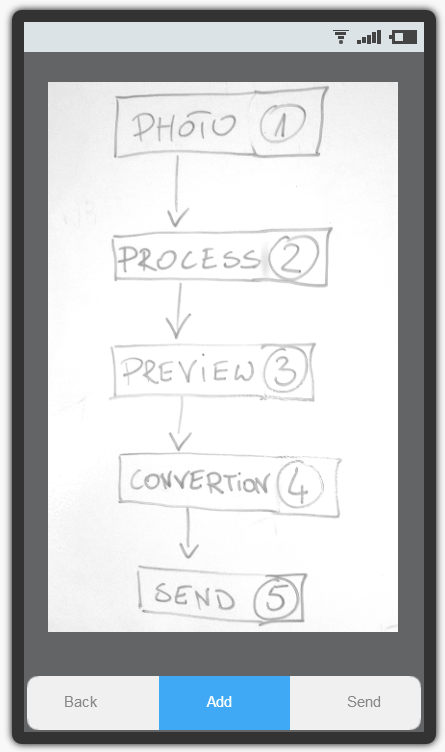
\includegraphics[height=10cm]{ocr.png}\end{center}
}
{-}
{Mateusz Jaworski}
{1 semester}
{1-3}
\end{project}
%%%%%%%%%%%%%%%%%%%%%%%%%%%%%%%%%%%%%%%%%%%%%%%%%%%%%%%%%%%%%%%%%%%%%%%%%%%%%%%%%%%%%%
\begin{project}
{Augmented notification system}
{Composite solution for distributing notifications via light, sound and touch.}
{
The system could have a form of central controller with many different 
peripheral devices that would be used for handling notifications and alarms. 
The main aim is to present status of continuous integration server in a highly visible manner. 
Those peripheral devices could have a form of RGB lamps, signal lights (same as used for the traffic control) or usb rocket launchers.
}
{-}
{Mateusz Jaworski}
{1 semester}
{1-4}
\end{project}
%%%%%%%%%%%%%%%%%%%%%%%%%%%%%%%%%%%%%%%%%%%%%%%%%%%%%%%%%%%%%%%%%%%%%%%%%%%%%%%%%%%%%%
\begin{project}
{Knowledge-based Expert System simulation environment}
{Ready to use simulation environment with CLIPS production system implemented.}
{
Knowledge-Based Expert System (KBES) is an artificial intelligence branch used for defining human-like reasoning, i.e. decision-making. The goal of the project is to integrate CLIPS system with some simulation environment (e.g. MATLAB), propose the object to be controlled, and define some set of production rules to test, whether it works fine enough. }
{C, C++, MATLAB, CMake, general AI knowledge}
{Pawel Ptasznik}
{1 semester}
{1-2}
\end{project}
%%%%%%%%%%%%%%%%%%%%%%%%%%%%%%%%%%%%%%%%%%%%%%%%%%%%%%%%%%%%%%%%%%%%%%%%%%%%%%%%%%%%%%
\begin{project}
{Eclipse plugin - Logs parser}
{
Implement Eclipse plugin that parses project source code for logs printings.
After loading of log file plugin is capable to jump into source code to point
the place where log was printed.
There are many applications in the world that generate logs in text format. It is difficult to find quickly where given log message comes from. 
}
{
 \begin{itemize}
  \item[-] Plugin for Eclipse to index code and parse logs
  \item[-] UI Eclipse configuration front-end
  \item[-] Jump into code after selecting particular log line
  \item[-] Ability to filter the log file after applying set of filters
\end{itemize}
}
{
 \begin{itemize}
  \item[-] Configurable log format
  \item[-] Configurable log print functions in code (allow support standard and custom print functions)
  \item[-] Jump into code after selecting particular log line
  \item[-] Support for C/C++ or other languages
\end{itemize}
}
{Grzegorz Kokot}
{2 semesters}
{2-6}
\end{project}
%%%%%%%%%%%%%%%%%%%%%%%%%%%%%%%%%%%%%%%%%%%%%%%%%%%%%%%%%%%%%%%%%%%%%%%%%%%%%%%%%%%%%%
\begin{project}
{Acceptance tests framework for JS-heavy web applications}
{Web testing framework for acceptance tests in natural language (similar/based
on Cucumber) for JS-heavy (AJAX) web applications.} 
{ 
Example:\newline\newline
\verb|OPEN http://www.nsn.com\newline 

TYPE 'hello' INTO .login-input\newline
TYPE 'pasword' INTO .pass-input\newline
CLICK input[type=submit]\newline

ASSERT SUCCESS\newline
ASSERT .status CONTAINS 'welcome'\newline 
ASSERT .main-page IS VISIBLE
}
{Java/C\#/Python/JS}
{Mateusz Jaworski}
{1 semester}
{1-3}
\end{project}
%%%%%%%%%%%%%%%%%%%%%%%%%%%%%%%%%%%%%%%%%%%%%%%%%%%%%%%%%%%%%%%%%%%%%%%%%%%%%%%%%%%%%%
\begin{project}
{Jenkins: deployment plugin}
{Plugin for web applications deployment} 
{ 
After build:
\begin{itemize}
\item[-] connect via ssh with remote server
\item[-] copy and unzip selected artefacts
\item[-] run script externally
\end{itemize}
}
{NodeJS/Python/Java}
{Wojciech Stachowski}
{1 semester}
{1-2}
\end{project}
%%%%%%%%%%%%%%%%%%%%%%%%%%%%%%%%%%%%%%%%%%%%%%%%%%%%%%%%%%%%%%%%%%%%%%%%%%%%%%%%%%%%%%
\begin{project}
{Jenkins build trigger}
{Jenkins plugin for builds triggering based on result of database query} 
{ 
Jenkins periodically queries the database, builds are triggered when query result matches given condition
}
{Support for PostgreSQL, MongoDb}
{Jacek Tomasiak}
{1 semester}
{1-2}
\end{project}
%%%%%%%%%%%%%%%%%%%%%%%%%%%%%%%%%%%%%%%%%%%%%%%%%%%%%%%%%%%%%%%%%%%%%%%%%%%%%%%%%%%%%%
\begin{project}
{Performance tests plugin for Jenkins}
{Jenkins plugin for execution and visualisation of performance tests' results} 
{ 
\begin{itemize}
\item[-] runs JUnit tests marked with @Performance annotation
\item[-] generates report in xml format
\item[-] presents results on CI server
\end{itemize}
}
{Preferred language: Java (JUnit)}
{Mateusz Jaworski}
{1 semester}
{1-2}
\end{project}
